\documentclass[a4paper,english, oneside, 12pt]{memoir} %kan laves til twoside
\chapterstyle{southall}
\usepackage[T1]{fontenc}
\usepackage[applemac]{inputenc}
\usepackage[english]{babel}
\usepackage{amsmath,amssymb,amsthm}
\numberwithin{equation}{section} 
\usepackage{booktabs,dcolumn,cellspace}
\usepackage{graphicx} %[pdftex]
\usepackage{wrapfig}
\usepackage{placeins} %float barrier
\usepackage[margin=3cm]{geometry} 
\setsecnumdepth{subsubsection}
\setcounter{tocdepth}{2}
\linespread{1.0}
\usepackage{array,booktabs}
\usepackage{caption}
\usepackage{subfig}
\usepackage{lscape}
\usepackage{array}
\usepackage{pbox}
\usepackage{lastpage}
%\usepackage{rotfloat}
\usepackage{multirow}
\usepackage{color}
\usepackage{relsize} 
\usepackage{fancyvrb}
\usepackage{tabularx}
%\usepackage{microtype}
\usepackage{rotating}
\usepackage{framed}
\usepackage{longtable}
\setlength{\parindent}{0pt}
\nonzeroparskip
\usepackage{lipsum}
\usepackage{listings}
\usepackage{algpseudocode}
\usepackage{textcomp}
\usepackage{hyperref}
\hypersetup{linktocpage}
\hypersetup{colorlinks,citecolor=red,filecolor=blue,linkcolor=red,urlcolor=blue}
\captionsetup[subfigure]{margin=10pt, parskip=0pt,hangindent=0pt, indention=0pt, singlelinecheck=true} 
\captionsetup[figure]{format=hang,justification=raggedright} %ndrer p caption pakken
\captionsetup{format=hang,justification=raggedright} %ndrer p caption pakken
\captionsetup[figure]{font={footnotesize,sf},labelfont=bf, singlelinecheck=1, width=0.85\textwidth}
\captionsetup[figure]{labelfont={bf,small},textfont={small}}
\captionsetup[subfloat]{labelfont={bf,small},textfont={small},
subrefformat=parens}
\usepackage{lineno}
\usepackage{minted}
\providecommand{\inlinecode}[1]{\texttt{\allowbreak#1}}
\providecommand{\todo}[1]{\addcontentsline{tdo}{todo}{\protect{#1}}\marginpar{\textcolor{red}{#1}}}
\newcommand{\tab}[1]{\hspace{.2\textwidth}\rlap{#1}}
\newcommand{\myparagraph}[1]{\paragraph{#1}\mbox{}\\}
\definecolor{listinggray}{gray}{0.9}
\definecolor{lbcolor}{rgb}{0.9,0.9,0.9}
\lstset{
  backgroundcolor=\color{lbcolor},
  tabsize=4,
  rulecolor=,
  language=matlab,
  basicstyle=\scriptsize,
  upquote=true,
  aboveskip={1.5\baselineskip},
  columns=fixed,
  showstringspaces=false,
  extendedchars=true,
  breaklines=true,
  prebreak = \raisebox{0ex}[0ex][0ex]{\ensuremath{\hookleftarrow}},
  frame=single,
  showtabs=false,
  showspaces=false,
  showstringspaces=false,
  identifierstyle=\ttfamily,
  keywordstyle=\color[rgb]{0,0,1},
  commentstyle=\color[rgb]{0.133,0.545,0.133},
  stringstyle=\color[rgb]{0.627,0.126,0.941},
}

\makepagestyle{plain}
\makeevenfoot{plain}{}{\thepage\ of \pageref*{LastPage}}{}
\makeoddfoot{plain}{}{\thepage\ of \pageref*{LastPage}}{}


\renewcommand\chapterheadstart{\vspace*{-1 pt}}
\renewcommand\listingscaption{Example}
\def\listingautorefname{example}
\renewcommand\figureautorefname{figure}

\pagestyle{plain}


\begin{document}

\frontmatter
\begin{titlingpage}

\centering \parindent=0pt
\newcommand{\HRule}{\rule{\textwidth}{1mm}}
\vspace*{\stretch{1}} \HRule\\[1cm]
\Huge\bfseries TAPY\\[0.7cm]
\large Type Analysis for Python \\[1cm]
\HRule\\[2cm] \large Jesper Lindstr\o m Nielsen - \textit{jesper.jln@gmail.com} \\
\large Christoffer Quist Adamsen - \textit{christofferqa@gmail.com} \\
\large Troels Leth Jensen - \textit{troelslethjensen@gmail.com} \\

\vspace*{2 cm}  \normalsize 

\begin{flushleft}
Aarhus University\\
May 3, 2013 \end{flushleft}




\end{titlingpage}

%\tableofcontents

\mainmatter
\chapter*{Abstract}
We present a proof of concept for doing type analysis for Python using the monotone framework. We present how some interesting language features are converted into control flow graphs (CFGs), and also how it is possible to dynamically extend a CFG with calls to the so-called magic methods during the analysis, in order to minimize the total CFG in which the analysis works on. Finally, we show that our type analyser is able to analyse small programs that involves non-trivial language features that distinguishes Python from other dynamic languages, e.g. JavaScript.
\chapter{Introduction}
Python is a dynamically typed, general purpose programming language that supports both object-oriented, imperative and functional programming styles.

Python has a lot of similarities to JavaScript as they are both dynamic languages. However, static type analysis of Python is further complicated by its scoping rules \cite{lambdapy}, magic methods, generator expressions and others. One of the reasons why magic methods are challenging to reason about, is that they result in implicit method and function calls; this makes it harder to predict the outcome of, otherwise relatively, simple statements and expressions, e.g. attribute lookup.

Python is widely used in both education and industry, and because of this popularity IDEs \cite{ide.appcelerator, ide.jetbrains, ide.wingware} and other third-party tools \cite{tool.pep8, tool.pyflakes, tool.pychecker, tool.pylint} have been developed to accommodate the developer by finding errors and making refactorings. Sadly, all these tools are affected by the complexity in the Python language and shown to be unsound \cite{lamdapy}. In this report we present our work towards developing a conservative and sound type analysis for Python version 2.7.5\footnote{This version is still predominantly used in the wild.} written in Scala, furthermore we use the third-party project Jython \cite{jython} to parse Python.

\section{Aims and Contributions}
Inspired by Type Analysis for JavaScript (TAJS) \cite{tajs} our aim for this project is to develop a type analysis for Python that will be able to analyze simple Python programs for type related errors. Especially, we wish to be able to do type analysis on programs that use the magic method \inlinecode{\_\_getattr\_\_}, which is called whenever an attribute lookup results in an \inlinecode{AttributeError}. In order to achieve this goal our type analyzer should be able to handle declarations and instantiations of classes, exceptions and others.

This report presents a proof of concept that static analysis of Python is possible using the traditional monotone framework. We present how to construct CFG snippets for various statements and expressions, including a dynamic way to change the CFG during execution of the analysis to accommodate the support for the magic method \inlinecode{\_\_getattr\_\_}.  

During the development of our project we have identified some intriguing features in Python, that includes its scope rules and the order of evaluation when handling magic methods.

\section{Dynamic features and type related errors}
\label{Features}
In this section we give some examples of typical type errors that may occur in Python programs.

Classes can be modified after creation. The code in \autoref{code:Features1} declares a class \inlinecode{Student} with a constructor that inherits from the builtin class \inlinecode{object}.

\begin{listing}[H]
  \begin{minted}[linenos]{python}
class Student(object):
  def __init__(self, name):
    self.name = name
s1 = Student('Foo')
s2 = Student('Bar')
def addGrade(self, course, grade):
  self.grades[course] = grade
Student.addGrade = addGrade
s1.grades = {}
s1.addGrade('math', 10)
s2.addGrade('math', 7)
  \end{minted}
  \caption{Magic method example in Python}
  \label{code:Features1}
\end{listing}

At line 8 a function \inlinecode{addGrade} is written to the \inlinecode{addGrade} attribute of the \inlinecode{Student} class. Since it is written onto a class it will be wrapped in an unbound method; this will ensure that the function can be called as a method on instance objects; especially, the receiver object will be implicitly passed to the \inlinecode{self}\footnote{The first argument is not required to be called \inlinecode{self}, but it is considered bad practice to name it otherwise.} argument (eliminating the purpose of having the \inlinecode{this} keyword as in e.g. JavaScript).

At line 9 the attribute \inlinecode{grades} is set to an empty dictionary on the \inlinecode{s1} object. Therefore we can call the (bound) method \inlinecode{addGrade} on the \inlinecode{s1} object without getting a runtime error. However, since we forgot to set the \inlinecode{grades} attribute on the \inlinecode{s2} object, we will get the following runtime error from line 11: \inlinecode{AttributeError:\ 'Student' object has no attribute 'grades'}. 

Recall that the receiver object is given implicitly as a first argument to the \inlinecode{addGrade} method. 
In case we had forgotten to supply the extra formal parameter \inlinecode{self}, the following runtime error would result from line 10:
\inlinecode{TypeError:\ addGrade() takes exactly 2 arguments (3 given)}. 

% Another interesting aspect with regards to parameter passing is that Python supports unpacking of argument lists. For instance we could have provided the arguments to the \inlinecode{addGrade} function in line 10 by means of a dictionary instead: \inlinecode{s1.addGrade(**\{ 'course': 'math', grade: 10\})}.

However, a type error would occur if line 9 was changed to \inlinecode{s1['grades'] = \{\}} (as is possible in JavaScript), namely: 
\inlinecode{TypeError:\ 'Student' object does not support item assignment}. Additionally, trying to access \inlinecode{s1['grades']} would result in the following error: \inlinecode{TypeError:\ 'Student' object has no attribute '\_\_getitem\_\_'}. Instead this could be achieved by calling the built-in functions \inlinecode{getattr(obj, attr)} and \inlinecode{setattr(obj, attr, val)}.

Python does however allow the programmer to customize the behavior when indexing into an object by supplying the magic methods
\inlinecode{\_\_setitem\_\_} and \inlinecode{\_\_getitem\_\_}, giving the programmer much more freedom. As an example consider the new Student class below:

\begin{listing}[H]
\begin{minted}[linenos]{python}
class Student(Person):
  def __getitem__(self, name):
    return self.grades[name]
  def __setitem__(self, name, val):
    setattr(self, name, val)
  def __getattr__(self, name):
    if name in self.grades:
      return self.grades[name]
    else:
      return "<no such grade>"
\end{minted}
	\caption{Magic method example in python}
	\label{code:Features2}
\end{listing}

With this implementation we could set the \inlinecode{grades} attribute as in JavaScript: \inlinecode{s1['grades'] = \{\}} (due to the implementation of \inlinecode{\_\_setitem\_\_}), and get the grade of \inlinecode{s1} in the math course by calling \inlinecode{s1.math} (due to \inlinecode{\_\_getattr\_\_}) or \inlinecode{s1['math']} (due to \inlinecode{\_\_getitem\_\_}). This is exactly one of the reasons why Python is so difficult to statically analyze: even something as fundamental as attribute lookups possibly involves several method invocations.

As mentioned we want our type analyzer to support the magic method \inlinecode{\_\_getattr\_\_} which comes into play when accessing attributes on class instances, as we illustrated above. In the section about magic methods we describe in detail what exactly happens, together with our work towards supporting this particular magic method.
\chapter{Our Approach}

Our approach for this project is to use existing frameworks and techniques with proven qualities to analyse the Python source code, most notably the monotone framework. This chapter contains outlines of how these frameworks and techniques are adapted to fit the specific task.

\section{Monotone framework implementation}

To get started an implementation of the monotone framework that is decoupled from the actual analysis was made. This implementation counts commonly used lattice structures, the worklist algorithm, a graph structure and an analysis interface (or trait in scala-lingo).

\subsection{Lattices}

In order to make our lives easier when constructing the actual analysis lattice, we have implemented several common lattice structures as type generic classes. These common lattice structures include, among others, a map and product lattice. In this section we will briefly go over the implementation decisions made for these structures.

Using classic object-oriented programming principles each of these compound structures decide the ordering of their elements by delegating to the underlying lattices in a point wise fashion, e.g. the product lattice has two underlying lattices, one for each element and thus the ordering is decided by comparing the first element in the pair in the context of the first lattice and similarly for the second element.

The map lattice has received a couple of changes from the naive implementation to make it usable in more cases. The first change was to interpret an unbound key value, $k$, to be a mapping from $k$ to the bottom element of the underlying lattice. In some use cases, such as a functional approach to intraprocedural static analysis, the map lattice will have a huge amount of keys. Requiring all of these to be bound to some value in the map is superfluous. This invariant is hidden completely in the lattice class because you can't manipulate the lattice element directly, so when trying to lookup an unbound key, the lattice simply constructs a fresh bottom value.

Since we now have a way to avoid binding every value from the key set, we are also able to change the constructor from the straightforward approach \inlinecode{s: Set[T], l: Lattice[S]} into a more general \inlinecode{s: T, l: Lattice[S]} (where \inlinecode{S} and \inlinecode{T} are type arguments)\todo{What is s and l? Explain...}. The straightforward approach has to compute the entire key set before you are able to instantiate the map lattice, but since the key set in itself might be exponentially large that wouldn't be practical. The downside to this change is, that since the map lattice has no way to know the intended key set, there is no way to construct the top element of the lattice.

% The top element of the lattice is useful for when you want to give up in the analysis, so to fix we instrumented the map lattice with a new top element, in a similar fashion to how the sink lattice instruments the underlying lattice with a new bottom element.

\subsection{Constraints}

Being in a functional programming language an easy-to-work-with representation of the constraints is anonymous lambda functions with the type \inlinecode{E $\rightarrow$ E}, where \inlinecode{E} is the type of the elements in the analysis lattice. Each constraint captures the node it was made from in its closure, so it is able to lookup the needed information in the lattice element.

This approach follows the notation very nicely, and as such makes the implementation a simple task when the constraints have been formulated formally.

\subsection{Worklist}
Our worklist implementation hasn't seen any optimizations and is as such just the straightforward implementation. First it generates constraint functions for each of the nodes in the CFG, adding each node to a worklist as it goes along. It then starts recursion (Scala benefits from tail call optimization to prevent the stack from exploding) on the list, popping one node from the list at a time. When a node is popped the corresponding constraint function is applied to the solution. Using Scalas built-in structural equality, the result is compared to the input and if they differ all nodes that depends on the popped node are added to the worklist.

A simple optimization would be to focus on finding a fixed-point for a strongly connected component of the CFG before continuing with the strongly connected components that depend on it, as also explained in section 5.1 from Static Program Analysis \cite{sa}.

\section{The Analysis Lattice}
Inspired by TAJS \cite{tajs} we have constructed a lattice for abstract values, $Value$ (see \autoref{lattice:Value}), from which we build a lattice for abstract objects, $Object$ (see \autoref{lattice:Object}). These two lattices are the main building blocks for the lattice of abstract states, $State$ (see \autoref{lattice:State}). Our analysis lattice is the lattice which for each program point (i.e. for each CFG node) describes the abstract state of that program point. Furthermore the $Analysis$ lattice (see \autoref{lattice:Analysis}) describes the call graph of the CFG.

\subsection{Abstract Values}
The lattice for abstract values follows below:

\begin{figure}[H]
\begin{eqnarray*}
Value = & Undefined \times None \times NotImplemented \times Ellipsis \\
        & \times Boolean \times Integer \times Float \times Long \\
        & \times Complex \times String \times P(ObjectLabel)
\end{eqnarray*}
\vspace{-15pt}
\caption{The $Value$ lattice.}
\label{lattice:Value}
\end{figure}

The $Value$ lattice is used to describe the abstract values of temporary variables, and attributes on objects. The $Undefined$, $NotImplemented$, $Ellipsis$ and $None$\footnote{\inlinecode{NotImplemented}, \inlinecode{Ellipsis} and \inlinecode{None} are examples of built-in constants. See \cite{pyref.constants} for a complete list of built-in constants in Python.} lattices all contain two nodes, top and bottom. $NotImplemented$ is a constant in Python which can be used when a function is not supported. $Ellipsis$ is another constant which represents \inlinecode{\dots} in Python; this constant can be used when indexing using intervals (also known as slicing). When a function does not contain a return statement, the constant \inlinecode{None} is returned by default, e.g.:

\begin{listing}[H]
	\begin{minted}[linenos]{python}
def a(): pass
a() is None # true
	\end{minted}
	\caption{Constant None}\label{code:NoneExample}
\end{listing}

Contrary to JavaScript, Python supports integers, floats, longs and complex numbers, so we have separate lattices for those. As lists in Python can only be indexed using integers our lattices does not have to keep track of whether a particular number is an unsigned integer or not, as the $Num$ lattice for TAJS does (page 8, \cite{tajs}). To TAJS it is crucial to have this distinction because the behavior of associative arrays are distinct based on whether an unsigned integer or not is used to index with. For the similar reason our $String$ lattice does not distinct between unsigned integer strings and arbitrary strings, as the $String$ lattice for TAJS does.

Note that $Complex = Float \times Float$, since a complex number in Python is represented using a float for the real and imaginary part, respectively \cite{pyref.stdtypes}. The $Integer$ lattice is defined here in \autoref{fig:latticeInteger}. The $Float$, $Long$ and $String$ lattices are defined in similar ways. Finally, a value can also be a pointer to an object on the heap, which we model in the $Value$ lattice by having a power set\footnote{All our power sets are ordered by subset inclusion.} of object labels, $P(ObjectLabel)$.

The notion of object labels will be described in \autoref{The Heap} about the heap.

\begin{figure}[H]
	\begin{center}
		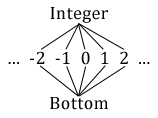
\includegraphics[width=0.25\textwidth]{images/integer-lattice.png}
	\end{center}
	\vspace{-15pt}
	\caption{The integer lattice}
	\label{fig:latticeInteger}
\end{figure}



\subsection{Abstract State}
We use the following lattice to model abstract state:

\begin{figure}[H]
\begin{equation*}
State = Heap \times Stack
\end{equation*}
\vspace{-15pt}
\caption{The $State$ lattice.}
\label{lattice:State}
\end{figure}

Before we describe the $Heap$ (\autoref{The Heap}) and $Stack$ (\autoref{The Stack}) lattices, we need to look at the $Object$ lattice:

\begin{figure}[H]
\begin{equation*}
Object = (AttributeName \rightarrow Value \times Global) \times P(ObjectLabel^{*})
\end{equation*}
\vspace{-15pt}
\caption{The $Object$ lattice.}
\label{lattice:Object}
\end{figure}

Having made special lattices for the 'primitive' objects there is still a need to handle the more complex objects such as class instances and function objects. As with JavaScript you can augment objects with attributes at runtime, so the lattice needs to accommodate this dynamic behavior. We therefore use a map from attribute names to values. For some objects it is required to track the scope in which they were defined, to model the closure they are evaluated in. Additionally, variable scope objects will be modeled with abstract values of this type, and here the ability to mark variables as global is needed, indicating that writes to this variable should be done in the global variable scope object. Thus the object lattice is the product between object values and a static scope chain modeled as a list of object labels. The static scope chain is only present for function objects and describes the scope of the function at its declaration. It is used to properly update the scope chain when calling the function.

\subsection{The Heap}
\label{The Heap}

\begin{figure}[H]
\begin{equation*}
Heap = (ObjectLabel \rightarrow Object)
\end{equation*}
\vspace{-15pt}
\caption{The $Heap$ lattice.}
\label{lattice:Heap}
\end{figure}

The heap is modeled by a map from object labels to object values. During the execution of a program there may be unbounded many objects on the heap, which we must approximate with a finite representation. We do this by using an object label for each allocation site, i.e. each node in the CFG that may create a new object on the heap. This is commonly known as the \textit{allocation-site abstraction} \cite{recency,aopas} \todo{Naevne der er ulemper ved kun et allocation-site object. Vi kommer ind paa dette i Strong vs. Weak updates afsnittet. Perspektiver til Rec Abs}. Thus, our abstract heap lattice will only contain one object for each such allocation site.

As an illustrative example consider the following very simple program:

\begin{listing}[H]
	\begin{minted}[linenos]{python}
class C(): pass
x = []
for y in range(0,2):
  x.append(C())
x[0].a = 'a'
x[1].b = 'b'
	\end{minted}
	\caption{Imprecision introduced by allocation-site abstraction.}
\end{listing}

At runtime this example generates two different \inlinecode{C} objects with attributes \inlinecode{a} and \inlinecode{b}, respectively. Using the allocation-site abstraction only a single \inlinecode{C} object would be created on the abstract heap. As a consequence, when writing to the attribute \inlinecode{a} at line 5, this is in principle done on each object originating from the same allocation-site\footnote{In order to deal with this conservatively, it must of course be a weak update. We discuss strong and weak updates in \autoref{section:Strong or weak}.}. Thus an analysis for this code should conclude at the end that the attribute \inlinecode{a} of an object originating from line 4 might be undefined or \inlinecode{'a'} (similar for \inlinecode{b}).

As a side note we mention that the approach taken here is quite similar to the one taken in the Static Analysis course\footnote{See \url{http://cs.au.dk/SA}.}, where a couple of points-to analyses for Tiny Imperative Language (TIP) was described. There, \textit{Targets} was introduced as the possible set of allocations-sites, which for TIP is the pointer targets \inlinecode{malloc-i} for a given program (page 74, \cite{sa}).

In our type analyser we found it beneficial to distinguish between different types of object labels but still handle them in the same way in the heap. To achieve this we made several different subclasses to the object label, e.g. a function object label, which besides its name also holds a reference to the CFG node that is the entry node for that function.


\subsection{The Stack}
\label{The Stack}
The $Stack$ lattice is defined as:

\begin{figure}[H]
\begin{equation*}
Stack = (Register \rightarrow Value) \times P(ObjectLabel^{*})
\end{equation*}
\vspace{-15pt}
\caption{The $Stack$ lattice.}
\label{lattice:Stack}
\end{figure}

For each register, which can be thought of as a temporary variable, we specify the value of that particular register. Recall that we use registers in our intermediate representation, see \autoref{fig:callCfg} in \autoref{CFG calls} about CFG construction of function and method calls.

The power set $P(ObjectLabel^{*})$ specifies the objects on the dynamic scope chain $ObjectLabel^{*}$, i.e. the runtime stack. The head element in the scope chain determines which object on the heap, local variable writes should we written to. For instance we will have an object on the heap for each program, that models the module/top-level script environment \inlinecode{\_\_main\_\_} \cite{pyref.main} (this is what corresponds to the global object in JavaScript). Whenever an assignment to a variable occurs in the top-level scripting environment, e.g. \inlinecode{x=10}, the variable \inlinecode{x} is set as a attribute mapping to the integer 10 on the \inlinecode{\_\_main\_\_} object in the heap.

The dynamic scope chain is captured as the static scope chain whenever a class or function is declared. This new static scope chain is stored in the $Object$ lattice as seen in \autoref{lattice:Object}. The following example demonstrates this:

\begin{listing}[H]
	\begin{minted}[linenos]{python}
x = 10
def a():
  return x
a() # 10
x = 42
a() # 42
	\end{minted}
\caption{Scope example.}
\label{code:ScopeExample}
\end{listing}

For this example we will have the following objects on the abstract heap:

\begin{enumerate}
  \item The \inlinecode{\_\_main\_\_} object,
  \item The object of the function \inlinecode{a},
  \item The scope object of \inlinecode{a} (which is an object similar to the \inlinecode{\_\_main\_\_} object, i.e. an object where local variables are written onto).
\end{enumerate}

When calling the function the dynamic scope chain will be set to the static scope chain related to the function \inlinecode{a} in order to model Pythons static scoping. When the variable \inlinecode{x} is read, \inlinecode{x} is looked up in the scope chain; for this particular example \inlinecode{x} is found on the \inlinecode{\_\_main\_\_} object.

In the \autoref{Functions} we describe our work towards handling functions, this includes populating the call graph such that the CFG becomes interprocedural.

\begin{figure}[H]
\begin{eqnarray*}
CallGraph = & P(Node \times Node) \\
Analysis = & (Node \rightarrow State) \times CallGraph
\end{eqnarray*}
\vspace{-15pt}
\caption{The $CallGraph$ and $Analysis$ lattice.}
\label{lattice:Analysis}
\end{figure}
\chapter{Control Flow Graph construction}
\ref{chap:CFGConstruction}

\section{CFG construction for For and While loops}
\ref{sec:CFGConstructionLoops}
In this section we give examples of how we inductively generate the control flow graph of some essential language features. During this we will present the control flow graph nodes that we use, together with their semantics. \\
In Python, both for and while loops has an else branch, which is executed if the loop terminates normally (i.e. not using \inlinecode{break}).

\begin{listing}[H]
	\begin{minted}[linenos]{python}
"for" target_list "in" expression_list ":" suite 
["else" ":" suite]
	\end{minted}
	\caption{For-loop syntax according to the Python Language Reference}\label{code:forSyntax}
\end{listing}

\begin{listing}[H]
	\begin{minted}[linenos]{python}
for x in [1,2,3]:
  print x
else:
  print "not a break'ed exit"
	\end{minted}
	\caption{For-loop example}\label{code:forExample}
\end{listing}

\begin{wrapfigure}{r}{0.5\textwidth}
	\vspace{-20pt}
	\begin{center}
		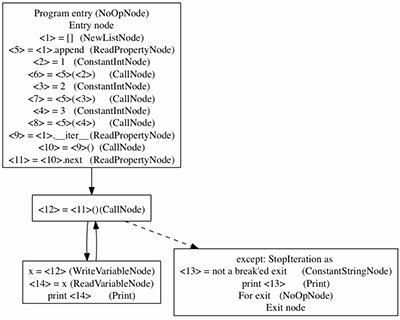
\includegraphics[width=0.48\textwidth]{images/for-example-cfg.png}
	\end{center}
	\vspace{-10pt}
	\caption{Control Flow Graph for the for-loop example \ref{code:forExample}}
	\label{fig:forCfg}
	\vspace{-10pt}
\end{wrapfigure}

First, \inlinecode{expression\_list} is evaluated. This should yield an iterable object, such that an iterator object can be created. Now for each element of the iterator the body of the for loop is evaluated once. As mentioned, if an else block is provided to the loop, it is evaluated when all iterations are done, and the iteration did not stop because of a break statement. \\
To simulate the evaluation sequence of such a for loop in our control flow graph, we need to take a look at the iterator object: to get the next element from a Python iterator object the next method is used. This method returns the next element until the iteration is done and finally raises a \inlinecode{StopIteration} exception. The CFG for the for-loop example \ref{code:forExample} can been seen in figure \ref{fig:forCfg}.

\begin{wrapfigure}{r}{0.5\textwidth}
	\vspace{-20pt}
	\begin{center}
		\includegraphics[width=0.48\textwidth]{images/while.png}
	\end{center}
	\vspace{-10pt}
	\caption{Control Flow Graph for a while-loop}
	\label{fig:whileCfg}
	\vspace{-10pt}
\end{wrapfigure}
For a while loop we generate the control flow graph in figure \ref{fig:whileCfg}.

\section{CFG cunstruction of With statements}
With statements in Python are unlike With statements in JavaScript.\ They are usually used when you have object you need to "open" before you do some work and then "close" it in the end, this pattern is used alot when working with I/O such as files or databases.\ An example of with statements can be seen in Listing \ref{code:withExample}.

\begin{listing}[H]
	\begin{minted}[linenos]{python}
with open('file.txt') as fh:
	print fh.read()
	\end{minted}
	\caption{With example reading a file}\label{code:withExample}
\end{listing}

The formal description of the With statement can be found in The Python Language Reference compound statement list\cite{pyref.compound} section 7.5, the hightlights is that if there is an \inlinecode{as} part of your with statement the result of the method call to \inlinecode{\_\_enter\_\_} assigned to the variable in the with statement. If there is raised an exception during the execution of the body of the With statement it is passed as arguments to the method call \inlinecode{\_\_exit\_\_}, if the result of that call returns something which truth value is \inlinecode{True} the with statement just evaluates normally, If a truth value of \inlinecode{False} is returned the exception isn't caught. If no exceptions happens during execution the \inlinecode{\_\_exit\_\_} method is called, after the body of the With statement, where \inlinecode{None} is passed as arguments.

\section{CFG construction of function and method calls}
\textit{CFG$_{\textit{cond}}$} is the control flow graph that results from the condition. If the condition is the boolean \inlinecode{True}, \textit{CFG$_{\textit{cond}}$} will be the control flow graph consisting of a single node, namely \textit{ConstantBooleanNode}. Inspired from TAJS, Type Analyzer for JavaScript, our \textit{ConstantBooleanNode} holds a result register (\textit{reg$_{\textit{cond}}$} in figure \ref{fig:callCfg}) together with the actual constant value, \inlinecode{True} in this case. \\
The other nodes \textit{ConstantIntNode}, \textit{ConstantFloatNode}, \textit{ConstantLongNode}, \textit{ConstantComplexNode}, \textit{ConstantStringNode}, \textit{ConstantNoneNode}, \textit{NewListNode}, \textit{NewDictionaryNode} and \textit{NewTupleNode} work in a similar way to \textit{ConstantBooleanNode}. \\
The motivation for introducing registers is that a single expression as e.g. \inlinecode{s1.addGrade('math', 10)} is evaluated in several steps. \\
First the function \inlinecode{addGrade} is looked up in the class of \inlinecode{s1}. This is done in the control flow graph using \textit{ReadPropertyNode}, which holds a result register, a base register, i.e. the register where to find the object, and the name of the property to look up. Similar nodes include \textit{ReadVariableNode} and \textit{ReadIndexableNode}. \\
\begin{wrapfigure}{r}{0.5\textwidth}
	\vspace{-20pt}
	\begin{center}
		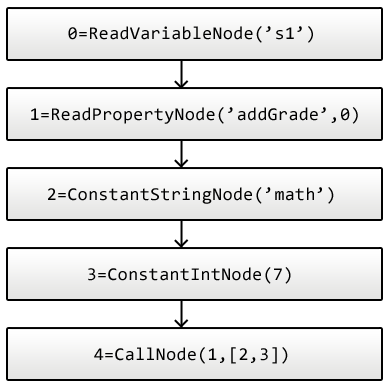
\includegraphics[width=0.48\textwidth]{images/Call-example.png}
	\end{center}
	\vspace{-10pt}
	\caption{Control Flow Graph for a call example}
	\label{fig:callCfg}
	\vspace{-10pt}
\end{wrapfigure}
Secondly, each argument given to the function is evaluated, and finally the actual call is done. Calls in the control flow graph is modeled using the \textit{CallNode}, which holds a result register, a function register and a list of arguments registers. \\
Thus the expression \inlinecode{s1.addGrade('math', 10)} will result in the control flow graph found in figure \ref{fig:callCfg} (where the numbers to the left represent the result registers of the nodes).\\
\todo{Tilfoeje afsnit om \_\_getattribute\_\_ og \_\_getattr\_\_, samt hvordan disse haandteres.} \\
So far we have primarily been concerned with putting constants into registers and reading e.g. variables. In order to support writing we have three different nodes: \textit{WriteVariableNode}, \textit{WritePropertyNode}, and \textit{WriteIndexableNode}. Besides holding a value register, i.e. the register where to find the value being written, \textit{WriteVariableNode} contains the name of the variable being written to, \textit{WritePropertyNode} contains a base register and the property being written to, and \textit{WriteIndexableNode} contains a base and property register (the latter has a register for the property because it is not constant, for instance we could write something like the following: \inlinecode{dict[getKey()] = aValue}, whereas property in \inlinecode{obj.property = aValue} must be a string).

\section{Handling exceptions}
In order to handle the flow caused by exceptions we use two different kinds of edges in the control flow graph. A solid edge indicates normal flow, and a dashed edge indicates exception flow. \\
In Python exceptions can be caught using a try-except-else-finally block. An except block can be annotated with a number of types, and each try-except-else-finally block may contain an arbitrary number of except blocks. As usual, the else block is entered in case of a normal exit, i.e. when no exceptions were raised inside the try block. \\
The AST provided by the Jython parser has been normalized from a try-except-else-finally block into a try-finally block, which contains a try-except-else block in its try block. \\
For instance the code in the first example \ref{code:tryExceptBefore} below is transformed into the code in the next example \ref{code:tryExceptAfter}:

\begin{listing}[H]
	\begin{minted}[linenos]{python}
try:
  <try-stms>
except Foo:
  <except-foo-stms>
except:
  <except-stms>
else: 
  <else>
finally:
  <finally>
	\end{minted}
	\caption{A try-except-else-finally example before convertion}\label{code:tryExceptBefore}
\end{listing}

\begin{listing}[H]
	\begin{minted}[linenos]{python}
try: 
  try:
    <try-stms>
  except Foo:
    <except-foo-stms>
  except:
    <except-stms>
  else:
    <else-stms>
finally:
  <finally-stms>
	\end{minted}
	\caption{A try-except-else-finally example after convertion}\label{code:tryExceptAfter}
\end{listing}

Inductively, CFG's for the statement lists <\inlinecode{try-stms}> (\textit{CFG$_{\textit{try}}$}), <\inlinecode{except-foo-stms}> (\textit{CFG$_{\textit{except-foo}}$}), <\inlinecode{except-stms}> (\textit{CFG$_{\textit{except}}$}), <\inlinecode{else-stms}> (\textit{CFG$_{\textit{else}}$}), and <\inlinecode{finally-stms}> are created. \\
The CFG for the finally block is then cloned into three duplicates (\textit{CFG$_{\textit{finally-normal}}$}, \textit{CFG$_{\textit{finally-handled-exc}}$}, \textit{CFG$_{\textit{finally-unhandled-exc}}$}). The purpose is to have one finally block for each of the following cases: 

\begin{enumerate}
  \item when no exceptions occur during the try block,
  \item when an exception is raised and caught by one of the surrounding except blocks, and no exception is raised from inside that except block, and
  \item when an exception is raised but not caught, which is the case when a) an exception is raised from
the try block and no except blocks handles this particular exception, b) an except block catches an exception raised by the try block, but then raises a new exception on its own.
\end{enumerate}

In particular, it is important that the finally block for handling case (3), i.e. \textit{CFG$_{\textit{finally-unhandled-exc}}$}, is not connected to the exit node of the try-except-else-finally block. Instead, it should be connected to its nearest surrounding except block (if any), or no except block at all (indicating that the program crashes with a runtime error because of an unhandled exception). \\
In the following sections we present the way we generate the CFG of a try-except-else-finally block.

\subsection{The try block}
Each node in \textit{CFG$_{\textit{try}}$} (that does not already have an outgoing exception edge) is connected using an exception edge to the entry node of the first except block (*), in this case the entry node of \textit{CFG$_{\textit{except-foo}}$}. We do not add exception edges to nodes that already have an exception edges, because this would be a loss of information: the control flow always goes to the nearest enclosing except block in case of exceptions. \\
The above models that if an exception occurs during evaluation of one of the statements in a try block, then the control flow will proceed from the first except block. \\
If there is no except blocks, each node should instead be connected using an exception edge to the entry node of its nearest surrounding except or finally block (specifially \textit{CFG$_{\textit{finally-unhandled-exc}}$}). However, we don't add any exception edges here; these will be added inductively because of (*) in case there are any surrounding except or finally blocks.

\begin{wrapfigure}{r}{0.5\textwidth}
	\vspace{-20pt}
	\begin{center}
		\includegraphics[width=0.48\textwidth]{images/Try-except-else-finally.png}
	\end{center}
	\vspace{-10pt}
	\caption{Control Flow Graph for try try-except example \ref{code:tryExceptAfter}}
	\label{fig:tryExceptCfg}
	\vspace{-10pt}
\end{wrapfigure}
\subsection{The except block}
The entry node of each except block is connected using an exception edge to the entry node of the next except block (except for the last block, of course). Thus we make an exception edge from the entry node of \textit{CFG$_{\textit{except-foo}}$} to the entry node of \textit{CFG$_{\textit{except}}$}. \\
We do this because the first except block might not catch the exception (because of the type restrictions), in which the control flow proceeds at the next except block. \\
Furthermore, each node inside the except block should be connected using an exception edge to the entry node of its nearest surrounding except or finally block (specifically \textit{CFG$_{\textit{finally-unhandled-exc}}$}). As above, this is handled inductively. \\
Finally, if an except block actually catches the exception, and no exceptions occur inside that except block, the control flow proceeds to the surrounding finally block (in this case, \textit{CFG$_{\textit{finally-handled-exc}}$}). 

\subsection{The else block}
If no exceptions occur, the else block should be evaluated. Thus we add a normal flow edge from the exit node of \textit{CFG$_{\textit{try}}$} to the entry node of \textit{CFG$_{\textit{else}}$}.\\
Since exceptions may result from evaluating the statements in the else block, each node in \textit{CFG$_{\textit{else}}$} should also be connected to the entry node of the nearest surrounding except or finally block (again, \textit{CFG$_{\textit{finally-unhandled-exc}}$}). \\
In case the evaluation of the statements in the else block does not raise any exceptions, the control flow proceeds either to the exit node of the whole try-except-else block, or in case there is a surrounding finally block, to the entry node of \textit{CFG$_{\textit{finally-normal}}$}.
\chapter{Analysing Functions}
\label{Functions}
In this chapter we motivate why the analyser puts two objects on the abstract heap for each function declaration, as mentioned in \autoref{The Stack}. One being the function object, and the other being the function scope object. The function object is necessary as functions are themselves objects, just like in JavaScript. For instance we can set an attribute on a function object:

\begin{listing}[H]
	\begin{minted}[linenos]{python}
def foo(): pass
foo.attr = 42
	\end{minted}
\caption{Setting an attribute on a function object.}
\label{code:FunctionPropertyExample}
\end{listing}

%Another thing with regards to function objects on the heap, is that Python has a built in method \inlinecode{\_\_call\_\_} on each function. This method is a function wrapper of the function itself; calling it will result in calling the function itself. We therefore map the attribute \inlinecode{\_\_call\_\_} on the function object to its function wrapper object. The following illustrates how each newly declared function has this method:

%\begin{listing}[H]
%	\begin{minted}[linenos]{python}
%def a():
%	print "a"
%a() // "a"
%a.__call__ # <method-wrapper '__call__' of function object at ...> 
%a.__call__() # "a"
%	\end{minted}
%\caption{On a newly declared function the \_\_call\_\_ attribute is set to a built in method wrapper.}\label{code:printFunctionExample}
%\end{listing}

%It is important to distinguish between the object of the function, and the function object, since \inlinecode{\_\_call\_\_} is not just a reference to the object of the function, as illustrated below:

%\begin{listing}[H]
%	\begin{minted}[linenos]{python}
%def a(): 
%	pass
%
%# TypeError: 'method-wrapper' object has only read-only attributes
%a.__call__.prop = 10
%	\end{minted}
%\caption{Function object and \_\_call\_\_ example}
%\label{code:callPropertyExample}
%\end{listing}

The function scope object is necessary as local variables inside a function should not be set as attributes on the function object (see \autoref{code:callPropertyExample}). In the analysis only one function scope object is created on the abstract heap. This is an abstraction since at runtime a new function scope object is created for each invocation of a particular function. This abstraction makes it possible to create the function scope object in our analysis when the function is declared.

A better abstraction would be to create a new function scope object for each call site. This is in fact what TAJS \cite{tajs} does. However, this abstraction has the same precision issues when faced with recursive functions.

No matter which abstraction is used, there is a potential for the precision of the analysis to be ruined, because all local variable writes must be modelled as weak updates to preserve soundness. This is discussed in \autoref{section:Strong or weak} about strong and weak updates.

\begin{listing}[H]
	\begin{minted}[linenos]{python}
def foo(): 
  x = 42
foo.x # AttributeError
	\end{minted}
\caption{Function object and \_\_call\_\_ example}
\label{code:callPropertyExample}
\end{listing}

\newpage

\section{Calling functions and updating the call graph}
A function call is represented by a \textit{CallNode} and an \textit{AfterCallNode} in the CFG.

If the register being called points to a function $f(p_1, ..., p_n)$, the function scope object of $f$ is found on the abstract heap, which is needed to handle parameter passing. For each parameter $p_i$ of $f$ we set $p_i$ as an attribute on the scope object of $f$ to the abstract value of the $i$'th supplied argument. This implies that reading the variable $p_i$ inside the function will yield the $i$'th supplied argument. 

In Python default arguments are supported. This is handled in the analysis by evaluating the default arguments in the CFG whenever a function is declared. The abstract values of the default arguments are saved in a list of registers which is used as standin for absent arguments when the particular function is called.

If the function is called more than once with different parameters, reading the $i$'th argument inside the function will result in the least upper bound of all $i$'th supplied arguments because we have no context sensitivity\footnote{In \cite{sa} it is described how the call string and functional approach can be used to obtain context sensivity.}. The following example illustrates this:

\begin{listing}[H]
	\begin{minted}[linenos]{python}
def f(p1): 
  return p1
f(10)
x = f(20) # x becomes the top element of the integer lattice, not 20
	\end{minted}
\caption{A consequence of not having context sensitivity.}
\end{listing}

Next, we update the call graph by inserting call edges from the call node to the entry node of $f$ and from the exit node of $f$ to the after call node. This implies that the worklist of our fixed-point algorithm will be updated with the entry node of $f$, such that it will be reevaluated.

At the function entry node we change the dynamic scope chain to the static scope chain of the function as mentioned in \autoref{The Stack}, which is found in the function object on the abstract heap.

When the fixed-point algorithm has processed a function the after call node can read the return value of the function and store it on the stack. The return value is stored in a special fixed register. Whenever the analysis encounters a return node it writes the returned value to this special register using a weak update.

We discuss how two take care of interprocedural exception flow in \autoref{chapter:Exceptions}.

\section{Strong or weak updates of local variables}
\label{section:Strong or weak}
Since only one scope object is created for each function there is a big potential for precision loss because soundness dictates that all writes to local variables are modelled as weak updates, i.e. least upper bound between the current value and the new value. This is due to the fact that a scope object of a particular function might exist in more than one instance at runtime, as it is the case with recursive functions.

\begin{listing}[H]
	\begin{minted}[linenos]{python}
def foo(i):
  if i==10:
    return
  else:
    foo(i+5)
foo(0)
	\end{minted}
\caption{Simple recursive function.}
\label{code:SimpleRecursive}
\end{listing}

In \autoref{code:SimpleRecursive} three function scope objects would exist simultaneously for \inlinecode{foo} at runtime. However, our abstraction only has one object so it needs to model all values of $i$ in the same summary. The only way to do this is to take the least upper bound of these abstract values resulting in the top element of the $Integer$ lattice.

The problem only arises in the presence of recursive functions, so to enable the analysis to do strong updates a command-line flag is introduced to tell the analysis if it can assume no recursive functions occur. This was very fast to implement and allowed more time to focus on the magic methods, which on their own doesn't introduce any recursion.

Alternatively, the call graph could be inspected for loops in order to detect recursive functions. However since the call graph is built dynamically as a part of the analysis a recursive function might not appear as recursive at the current iteration possibly leading to strong updates, thus special care is needed when functions are labeled recursive.

An entirely different approach is to use the recency abstraction as introduced by \cite{recency}, which can be seen as an extension of the allocation-site abstraction. The idea is to allocate two objects for each allocation-site $s$, namely the most-recently-allocated-block (MRAB[$s$]) and not-most-recently-allocated-blocks (NMRAB$s$), instead of only one as in the allocation-site abstraction. This will allow for strong updates to attributes of MRAB[$s$]. This turns out to work very well because all writes to local variables at runtime happen to the latest instantiated stack frame, which is exactly the situation in which recency abstraction enables strong updates over weak updates.

\newpage

\section{Further work with parameter passing}
In Python it is possible to unfold e.g. a dictionary to the arguments of a function:

\begin{listing}[H]
	\begin{minted}[linenos]{python}
def foo(bar, baz):
	return bar + baz
params = { 'bar': 'bar', 'baz': 'baz' }
foo(*params) # 'barbaz'
	\end{minted}
\caption{Unfolding of a dictionary to the parameters a function.}
\label{code:UnfoldDictFunctionExample}
\end{listing}

Currently, our analysis does not support this kind of parameter passing. Also, it does not support the special \inlinecode{**args} parameter that collects all of the superfluous arguments in a list, quite similar to the \inlinecode{arguments} object that is available inside functions in JavaScript.
\chapter{Analyzing Classes}
Python has two different kinds of classes, namely new and old style (or classic) classes that both supports multiple inheritance (note that from Python 3 all classes are new style classes). A new style class is one that contrary to an old style class is a subclass of \inlinecode{object}. The two different kinds of classes vary among others in their method resolution order (MRO)\cite{pyref.typehierarchy}: old style classes resolves variables and attributes by a depth-first, left-to-right strategy, whereas new style classes uses the more complex strategy C3\cite{pyref.c3mro}, which is also known as the call-next-method from other multiple inheritance languages. Also, the built in function \inlinecode{super} can only be used with new style classes. In this section we present our work towards handling those two kinds of classes.

To start with consider the below example that illustrates the difference in MRO between new and old style classes.

\begin{listing}[H]
	\begin{minted}[linenos]{python}
class A():
	x = 'A'
class B(A): pass
class C(A):
	x = 'C'
class D(B, C): pass
D().x # 'A'
	\end{minted}
	\caption{Multiple inheritance}\label{code:OldStyleMROExample}
\end{listing}

Since \inlinecode{D} extends \inlinecode{B} and \inlinecode{C}, which in turn extends the old style class \inlinecode{A}, \inlinecode{D} is itself an old style class. Therefore, evaluating \inlinecode{D().x} will result in \inlinecode{'A'}. If we instead had declared \inlinecode{A} as a new style class \inlinecode{class A(object): ...}, evaluating \inlinecode{D().x} would result in \inlinecode{'C'}.


\section{Class declarations}
To start with we must take care of class declarations. In the CFG we have the following nodes related to this: \textit{ClassDeclNode}, \textit{ClassEntryNode}, and \textit{ClassExitNode}. Consider a class declaration like \inlinecode{class C(B1,...,Bn):<body>}. For this particular code we create a class declaration node in our CFG which holds the name of the class and the names of the baseclasses, i.e. \inlinecode{C}, and \inlinecode{B1}, ..., \inlinecode{Bn}. Furthermore we create a class entry node which we make the successor of the class declaration node. Then the inductively created CFG for the piece of code appearing at \inlinecode{<body>} will be inserted after the class entry node, and finally, we create a class exit node and make it the successor of the exit node of the inductively created \inlinecode{<body>} CFG.

More or less, the purpose of the three different kinds of nodes is the following:

\begin{itemize}
	\item The class declaration node, \textit{ClassDeclNode}, creates one or more class objects on the heap and writes the variable \inlinecode{C} as a property on each object that is on top of on of the scope chains.
	\item The class entry node, \textit{ClassEntryNode}, modifies the set of execution contexts by pushing the newly created class object on top of each of them.
	\item The class exit node, \textit{ClassExitNode}, reverts the execution contexts to what they were before visiting the class entry node (by popping the newly created class object from each of the execution contexts).
\end{itemize}

\subsection{Creating the class objects on the heap}
As mentioned our type analysis creates one or more class object on the heap whenever a class declaration node is meet. More precisely:

\begin{itemize}
	\item If \inlinecode{C} is definately a new style class a new style class object is created on the heap. Likewise for old style classes.
	\item Otherwise, both a new style class object and an old style class object is created on the heap.
\end{itemize}

For the example in listing \ref{code:OldStyleMROExample} our analysis will only create an old style class object on the heap, however for the below example we generate two objects.

\begin{listing}[H]
	\begin{minted}[linenos]{python}
if (...):
	class B(): pass
else:
	class B(object): pass
class C(B): pass
	\end{minted}
	\caption{An example where we can't conclude that \inlinecode{C} is definately a new style class or definately an old style class.}\label{code:NotDefinatelyNewOldStyleClass}
\end{listing}

We conclude that a class is definately a new style class if the following holds:

\begin{enumerate}
	\item The built in class \inlinecode{object} has not been overwritten.
\end{enumerate}

Of course it would still be possible to conclude that \inlinecode{class C(O): ...} is a new style class if the variable \inlinecode{O} has been set to \inlinecode{object} before overwriting \inlinecode{object} like in the below example.

\begin{listing}[H]
	\begin{minted}[linenos]{python}
O = object
object = 42
class C(O): pass
	\end{minted}
	\caption{The class \inlinecode{C} here is easily seen to be a new style class.}\label{code:ClassOverwrittenObject}
\end{listing}

However, our implementation does not at the moment check this because of the limited time of our project, and the fact that programmers should really not overwrite the built in \inlinecode{object}. Note that our implementation does conclude that \inlinecode{class C(O): ...} is a new style class if line 2 in the example had been skipped.

If \inlinecode{object} has not been overwritten, we check that:

\begin{enumerate}
\setcounter{enumi}{1}
	\item All the base classes \inlinecode{B1}, ..., \inlinecode{Bn} are either the built in object or definately a new style class.
\end{enumerate}

Recall that the baseclasses \inlinecode{B1}, ..., \inlinecode{Bn} are just variablenames. If \inlinecode{Bi} is the variable \inlinecode{object}, we can conclude that it is the built in object since we from (1) have that the built in \inlinecode{object} has not been overwritten. If \inlinecode{Bi} is not \inlinecode{object} we look up the variable on the scope chain, and make sure its value is only a pointer to a new style class object on the heap, or the built in class \inlinecode{object}. If it is for instance a pointer to either a new style class object or an old style class object (see for instance listing \ref{code:NotDefinatelyNewOldStyleClass}), we conclude that the class \inlinecode{C} it is not definately a new style class object.

In the same way we conclude that a class is definately an old style class.

\subsection{Populating the class objects on the heap with fields and methods}
As mentioned above the heap objects we create at class declaration nodes are empty. We add fields and methods to these heap objects inbetween the class entry and class exit nodes. First, let us investigate how fields and methods are created for classes below.

Fields and methods can be created at class declaration time, and dynamically added to the class after declaration as the following tries to illustrate:

\begin{listing}[H]
	\begin{minted}[linenos]{python}
class C(object):
	x = 10
	def getX(self):
		return self.x
def setX(self, x):
	self.x = x
C.setX = setX
	\end{minted}
	\caption{Adding a field \inlinecode{x} and methods \inlinecode{getX} and \inlinecode{setX} on a class.}\label{code:FieldAndMethodOnClass}
\end{listing}

We can handle this quite easily in our analysis by just updating the scope chains at class entry: we push the relevant class object on the heap (whether it is a new or an old style class) onto each current scope chain. As a result when we write to a variable like \inlinecode{x} inside the class it will be written to the head of each scope chain, i.e. the class heap object, which is exactly what we want.

This is however not quite enough in order to support methods since our CFG does not distinguish between function and method declarations. Thus \inlinecode{getX} will appear as a function declaration in our CFG, even though it is actually a method. We handle this at function declaration time by checking whether the head of the scope chain is a class object. In that case we wrap the function in an unbound method object, which is merely just a pointer to the function object. Otherwise we proceed as we would otherwise have handled a function declaration as explained in section \ref{Functions} about functions.

We wrap the function in an unbound method object for at least two reasons:

\begin{enumerate}
	\item It is not possible to write properties on methods, but properties on methods can be read in case the underlying function has the property.
\end{enumerate}

This is illustrated by the following example:

\begin{listing}[H]
	\begin{minted}[linenos]{python}
class C(object): pass

def foo(self): pass
foo.prop = 42

C.foo = foo
C.foo.prop # 42
C.foo.prop = 0 # AttributeError
	\end{minted}
	\caption{It is not possible to set properties on methods.}\label{code:FieldAndMethodOnClass}
\end{listing}

\begin{enumerate}
\setcounter{enumi}{1}
	\item When creating a class instance the unbound methods of the class are turned into bound methods on the instance object (we concentrate on this in the following section, Handling object creations).
\end{enumerate}

Fields and methods can also be added to a class after declaration time as was illustrated in example \ref{code:FieldAndMethodOnClass}. In our CFG this is represented by a \textit{WriteVariableNode}, so what we do in this case is very simular to what we do inbetween the class entry and exit nodes: if the object being written to is a class object, and the value being written is a function, then we wrap it in an unbound method object. Otherwise we just write the value to the property of the object as we would normally have done.


\subsection{Handling object creations}
When an instance of a class is created each unbound method of the class is turned into a bound method on the object. The purpose of the bound method is to pass the instance reference as the first argument to the unbound method (the \inlinecode{self} argument). As a consequence our lattice, unlike e.g. the lattice used by the TAJS Analyzer, does not contain an explicit representation of the \inlinecode{this} object (it is simply treated as a normal parameter to the function). The below example illustrates the implicit passing of the self parameter for bound methods:

\begin{listing}[H]
	\begin{minted}[linenos]{python}
class C(object):
	def foo(self):
		pass

C.foo # <unbound method C.foo>

x = C()
x.foo # <bound method C.foo of <C object at ...>>

x.foo() # self implicitly passed as self
C.foo(x) # using the unbound method by explicitly passing an instance

# TypeError: unbound method foo() must be called with C instance as 
# first argument (got nothing instead)
C.foo()
	\end{minted}
	\caption{Bound and unbound methods.}\label{code:BoundAndUnboundMethodsOnClass}
\end{listing}

Contrary to e.g. JavaScript, class instances are not created using the \inlinecode{new} keyword as can be seen from the above example. This means that we can't necessarily distinguish a function call from an object creation.

At each function call (i.e. \textit{ClassNode} in our CFG) we therefore investigate which kind of object label on the heap we are calling\footnote{It is of course a \inlinecode{TypeError} whenever the value being called is something that is not only a function object, a function wrapper object, a class object, or a method object}. If we happen to call a new style class object on the heap, we create a new style instance object on the heap, representing the newly created instance (likewise for old style classes). In particular, we do not modify the call graph as we do for function calls unless the magic method \inlinecode{\_\_init\_\_} has been implemented on the class (see the following section, Supporting constructor calls, on how we handle this).

Of course we wish generate the class instance objects conservatively. Consider the following code:

\begin{listing}[H]
	\begin{minted}[linenos]{python}
if (...):
	class C(): pass
elif (...):
	class C(object): pass
else:
	def C():
		return 42
x = C()
	\end{minted}
	\caption{Difference between methods and functions on classes.}\label{code:BothNewOldClassAndFunction}
\end{listing}

For this code we can't tell whether \inlinecode{C} after the \inlinecode{if} statement is the old style class in line 2, the new style class in line 4 or the function in line 6. Therefore, our analysis will conclude that \inlinecode{x} is either a pointer to a new style class instance, a pointer to an old style class instance, or the integer 42. This is seen in the figure below generated by our type analysis, which is the output of the heap at the exit node of the CFG of the code in example \ref{code:BothNewOldClassAndFunction}.

\begin{listing}[H]
	\begin{center}
		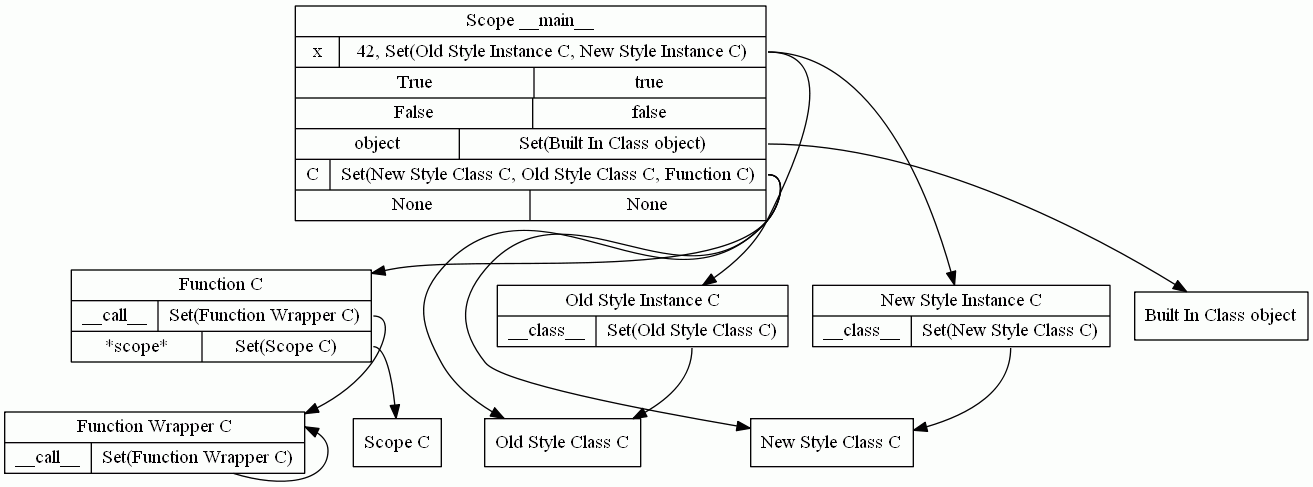
\includegraphics[width=1\textwidth]{images/BothNewOldClassAndFunction.png}
	\end{center}
	\vspace{-10pt}
	\caption{The heap generated by our analysis tool.}
	\label{fig:BothNewOldClassAndFunction}
\end{listing}

So far we haven't mentioned how we populate the newly created class instance object with the fields of the class, but this is more or less trivial: Each field (i.e. attribute) of the class is copied to the instance object, and each unbound method of the class is transformed into a bound method on the instance object (i.e. we create a new bound method object on the heap for each unbound method on the class).


\section{Supporting constructor calls}
The magic method \inlinecode{\_\_init\_\_} can be set on a class in order to supply a constructor as the following illustrates:

\begin{listing}[H]
	\begin{minted}[linenos]{python}
class C(object):
	def __init__(self, x):
		self.x = x

c = C(42)
c.x # 42
	\end{minted}
	\caption{The \inlinecode{\_\_init\_\_} magic method.}\label{code:InitConstructorClass}
\end{listing}

This introduces a minor issue that arises from the fact that we cannot at first sight distinguish between object creations and usual function calls (recall that Python has no \inlinecode{new} keyword). What happens at line 5 in example \ref{code:InitConstructorClass} above is the following:

\begin{enumerate}
	\item A new style instance object is created on the heap because of the call to a new style class object.
	\item A value pointing to this newly created instance object is stored in the special return register on the stack.
	\item The call graph is updated with call edges from the call node to the entry node of \inlinecode{\_\_init\_\_}, and from the exit node of \inlinecode{\_\_init\_\_} to the after call node.
	\item As a result of (3), the return value of \inlinecode{\_\_init\_\_} is stored in the special return register. Note that the return value of \inlinecode{\_\_init\_\_} must be the built in constant \inlinecode{None}; otherwise a type error results (for this example our CFG will insert an implicit return \inlinecode{None} node).
	\item The after call node will now read the value from the special return register on the stack and store it; in this case as the attribute \inlinecode{x} of \inlinecode{c}.
\end{enumerate}

For this approach the best we can do is to take the least upper bound when we write to the special return register. As a consequence the variable \inlinecode{c} from the example will after the object creation be set to the value corresponding to either being \inlinecode{None} or a new style instance object (meaning that we should report a type error in line 6, because a property is possibly being dereferenced on a non-object!).

We solve this issue by introducing a new special constructor return register, where we store newly created class instances in, together with a new kind of call edge in the call graph; constructor call edges.

The idea is the following: Instead of updating the call graph with call edges in (3), we update it with constructor call edges. This means that we can recognize returns from \inlinecode{\_\_init\_\_} functions, check that they are indeed \inlinecode{\_\_None\_\_} (otherwise raise a type error) and then ignore it.

Specifically, our implementation has a special join operation for after call nodes (for all other nodes the join operation just takes the least upper bound of the solutions of its predecessors). This join operation for after call nodes is the usual join operation, except that solutions coming from constructor call edges have their special return register (containing \inlinecode{\_\_None\_\_} emptied). As a consequence, our analysis can just take the least upper bound of the values in the special return and the special constructor return register, respectively, and store it in e.g. the attribute \inlinecode{x} of \inlinecode{c}.


\section{Further class work}
Not implemented yet: Resolution of methods and fields in super classes (specifically implementing the C3 MRO)\todo{Fixme}.

\section{Analyzing a concrete example}
Give a concrete example together with the output of our analysis tool on that particular example\todo{Fixme}.
\chapter{Exceptions}
\section{Raising exceptions intraprocedurally}
As it has not been our primary goal to fully support exception handling, but only to support some kind of simple exception handling in order to be able to handle the magic method \inlinecode{\_\_getattr\_\_}, we have only concentrated on except blocks (catch blocks) without types that catches all raised exceptions. In particular we don't support except blocks like \inlinecode{except AttributeError as e}.

As a consequence the changes to our type analyzer has been minor. When an exception is possibly raised the type analyzer writes that particular exception object to a special temporary variable where we store the latest raised exception. If the exception is raised by means of a \inlinecode{RaiseNode} in the CFG, the exception object will already be stored in a temporary variable. This is the case because the code \inlinecode{raise Exception()} is represented as follows in our CFG:

\begin{listing}[H]
	\begin{center}
		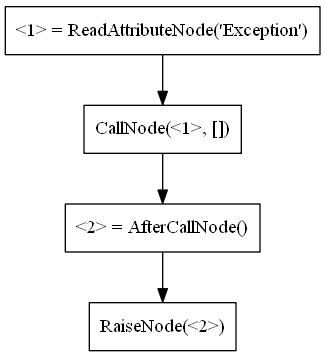
\includegraphics[width=0.4\textwidth]{images/raiseexception.png}
	\end{center}
	\vspace{-20pt}
\end{listing}

Therefore, our type analyzer can just take that object (for the example: the object in \inlinecode{<2>}) a store it in the temporary exception variable.

When an exception is not raised by means of a \inlinecode{RaiseNode}, our type analyzer creates a new exception object on its own. If for instance an attribute is read on an object without that attribute, we create a new \inlinecode{AttributeError} object and store it on the heap in our lattice. We do this as follows:

\begin{enumerate}
	\item The \inlinecode{\_\_builtin\_\_} module object on the heap is looked up,
	\item The attribute "AttributeError" is looked up on the \inlinecode{\_\_builtin\_\_} object from (1); this should always yield a \inlinecode{NewStyleClassObjectLabel},
	\item We manually create an instance of that particular class label found in (2), stores it on the heap of our lattice and finally also in the temporary exception variable on our stack lattice.
\end{enumerate}


\section{Raising exceptions interprocedurally}
The above outline only specifies how we raise exception intraprocedurally, since we so far haven't specified any exception edges in our CFG going across function definitions.

We take care of exceptions interprocedurally by introducing a new type of node for function exit: \inlinecode{ExceptionalExitNode}. Thus for each function we have two exit nodes. We now take each of the CFG nodes of the function that does not have an outgoing exception edge\inlinecode{If a CFG node in a function already has an outgoing exception edge, it is because it is inside a try-except block.} and connect them to the exceptional exit node by an exception edge.

Recall from the section about functions, that we upon a call to a function update the call graph with call edges from the call node to the entry node of the function, and from the exit node of the function to the after call node. In order to accommodate exceptions interprocedural we now also add a \textit{call exception edge} from the exceptional exit node of the function to the except block of the call node. To illustrate this consider the below example together with its corresponding (partial) CFG:

\begin{listing}[H]
	\begin{minted}[linenos]{python}
class C(object):
  if (trickyComputation()):
    a = 42
x = C()
def foo():
  result = x.a
  return result
try:
  y = foo()
except:
  err = "An error occured"
	\end{minted}
\end{listing}

\begin{listing}[H]
	\begin{center}
		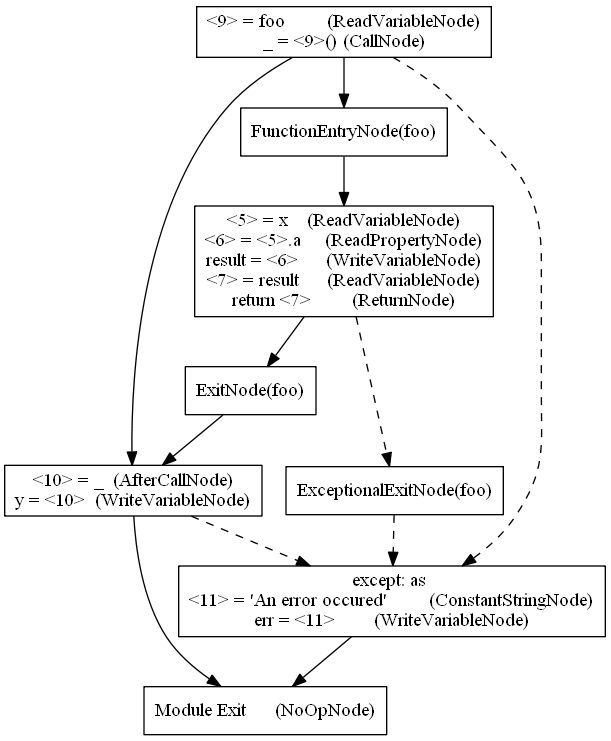
\includegraphics[width=0.75\textwidth]{images/exception1.png}
	\end{center}
	\vspace{-10pt}
\end{listing}


\section{Catching exceptions}
The constraint function for an \inlinecode{ExceptNode} in the CFG reads the value of the temporary variable associated with the latest raised exception. If the exception variable is bottom the solution of this node is simply set to the bottom element of the $State$ lattice. This indicates that the path is infeasible and acts as a simple sort of path sensivity. If the exception variable is actually set to an object on the heap, we just clear the exception variable on the stack by setting it to the bottom element of the $Value$ lattice. Now, the CFG nodes in the except block will change the solution as it looked like when an exception was raised, and the node following the try and except blocks will join the state coming from the try and except block, respectively.

As an example consider the following code:

\begin{listing}[H]
	\begin{minted}[linenos]{python}
class C(object):
  if (trickyComputation()):
    a = 42

x = C()
try:
  y = x.a
  z = "trickyComputation() was true"
except:
  err = "An error occured"
	\end{minted}
	\caption{An example that involves exceptions together with the solution of our type analyzer (see below).}
\end{listing}

Our type analyzer will for this particular code conclude that for the exit node of the program:

\begin{itemize}
	\item \inlinecode{y} is either undefined or 42
	\item \inlinecode{z} is either undefined or "trickyComputation() was true"
	\item \inlinecode{err} is either undefined or "An error occurred"
\end{itemize}

For the state at the last program point in the try block, our type analyzer concludes that:

\begin{itemize}
	\item \inlinecode{y} is undefined or 42
	\item \inlinecode{z} is "trickyComputation() was true"
\end{itemize}

\chapter{Results}
\label{chapter:results}
In this report we have presented one approach to a type analyser for Python, capable of analysing simple Python programs. In this chapter we will give examples of some small non-trivial programs together with the results from our type analyser. The primary goal was to support simple usage of the magic method \inlinecode{\_\_getattr\_\_} similar to the way it was used in Django \cite{django}.

%During our project we have developed a type analyser for Python, which is able to analyse simple Python programs. In this section we present some small, but non-trivial to %analyse, programs together with the results of our type analyser. We aimed to be able to support simple use of the magic method \inlinecode{\_\_getattr\_\_}, as we found that %all uses of it in the web framework Django\cite{django} were simple.

In order to achieve this goal limited support for exceptions was needed. Consider the following calculator example that makes use of exceptions for unsupported operations:

\begin{listing}[H]
	\begin{minted}[linenos]{python}
def calculator(a, op, b):
  if (op == "+"): result = a + b
  elif (op == "-"): result = a - b
  elif (op == "*"): result = a * b
  elif (op == "/"): result = a / b
  else: raise Exception()
  return result

try:
  amodb  = calculator(10, "%", 20)
except:
  err = "An error occured"
	\end{minted}
\end{listing}

For this example our analyser will conclude that \inlinecode{amodb} is undefined and that \inlinecode{err} is "An error occurred". Due to a very simple path sensitivity our analyser doesn't conclude that \inlinecode{amodb} is either undefined, \inlinecode{a}+\inlinecode{b}, \inlinecode{a}-\inlinecode{b}, \inlinecode{a}*\inlinecode{b} or \inlinecode{a}/\inlinecode{b}. By changing line 15 to \inlinecode{calculator(10, "+", 20)} our analyser would conclude that the result of the function call would be 30.

The limited exception handling has enabled us to support implicit \inlinecode{\_\_getattr\_\_} calls. Consider part of the \inlinecode{Student} example from \autoref{Features} about dynamic features that uses the magic method \inlinecode{\_\_getattr\_\_}:

\begin{listing}[H]
	\begin{minted}[linenos]{python}
class Student(object):
  def __init__(self, name):
    self.name = name
  def __getattr__(self, name):
    if name in self.grades:
      return self.grades[name]
    else:
      raise AttributeError()
a = Student('John')
a.grades = { 'math': 'A' }
try:
  mathgrade = a.math
except:
  err = "Error"
	\end{minted}
\end{listing}

Our tool is able to analyse this program and conclude that \inlinecode{mathgrade} is either \inlinecode{'A'} or \inlinecode{undefined} (the latter because we do a weak update in line 10 to \inlinecode{a.grades}). It should be mentioned, that the lack of context sensivity destroys the precision very quickly because Python has a lot of implicit method calls, contrary to JavaScript.

Dynamically expanding the \textit{ReadAttributeNode} results in 12 added CFG nodes per expanded \textit{ReadAttributeNode}, however it can be avoid when it can be statically determined that the attribute is definitely present. It would be nice to give a measure of how often the dynamic expansion can be avoided, but because our current analyser doesn't make any strong updates on classes it always does the expansion, except when we make use of the assumption mentioned in \autoref{Magic methods transformation}.

It is important to stress the fact that we only support a subset of Python. Not supporting the magic method \inlinecode{\_\_getattribute\_\_} simplifies the situation as discussed in \autoref{Magic methods transformation}.
\chapter{Limitations}

Rather than going with the latest version of Python, we will be working on version 2.7. This version is still predominantly used in the wild and we were only able to find a ready-to-use parser for 2.7 which, given the scope of this project, was a huge selling point. The magic methods remain unchanged in the 3.x family, so extending this proof of concept for a more recent version is straightforward.

\section{Language features}
Python is a general purpose programming language and quite popular, it has been developed and extended and holds a lot of different functionality, some of these functionalities is not used that often. In our analysis we have decided to exclude some of these language functionalities;

\begin{itemize}
	\item Lambda expressions
	\item Generator expressions
	\item Yield expressions
\end{itemize}

Each of these features present a great deal of complexity so to be able to go in depth with the magic methods these will remain unhandled. Thankfully these features don't seem to get used much either, so it should not hinder us is finding programs.

\todo{Exceptions, Imports}

\subsection{Function decorators}
In Python the decorator design pattern is built-in and when annotating a function it is possible to wrap it in another function. The typical use cases of this is when converting functions to methods and visa-versa. The description of decorators can be found in The Python Language Reference compound statement list\cite{pyref.compound} section 7.6. We have excluded this from our analysis.

\section{Numbers}
The size of an integer in Python depends on the system your on. If your running python on a x64 machine you will be able to create integers in the interval $[-2^{63}-2;2^{63}-1]$, where on a x86 machine your integers would be limited to the interval $[-2^{31}-2;2^{31}-1]$. These limitations is also described in The Python Language Reference data model\cite{pyref.datamodel} in section 3.2. In our analysis we assume that our target machine is a x86 and the integers is then limited to 32-bits.

\section{Magic methods}
Python uses magic methods to give the developer flexibility to do operation overloading on custom classes. These methods makes simple operations such as binary and unary operations hard to emulate in the control flow graph since its not just one operation but could potentially be a method-call with side-effects. \\
We have choosen to focus on the magic methods that is used when properties on an object is accessed. These methods is called \_\_getattribute\_\_ and \_\_getattr\_\_. A complete list and description on the magic methods can be found in The Python Language Reference data model\cite{pyref.datamodel} in section 3.4.

\begin{thebibliography}{8}

\bibitem{tajs} Simon Holm Jensen, Anders M\o ller and Peter Thiemann. Type Analysis for JavaScript. \url{http://www.brics.dk/TAJS/}.
\bibitem{sa} Anders M\o ller and Michael I. Schwartzbach. Static Program Analysis. Department of Computer Science, Aarhus University, Denmark. January 30, 2013.
\bibitem{lamdapy} Shriram Krishnamurthi and Joe Gibbs Politz et. al. Python: The Full Monty, submitted OOPSLA 2013 paper, March 28, 2013
\bibitem{jython} The Jyhton Project: Python for the Java Platform \url{http://www.jython.org/}, June 26, 2013
\bibitem{pyref.datamodel} The Python Language Reference, Datamodel \url{http://docs.python.org/2/reference/datamodel.html}, May 13, 2013
\bibitem{pyref.constants} The Python Language Reference, Constants \url{http://docs.python.org/2/library/constants.html}, May 13, 2013
\bibitem{pyref.stdtypes} The Python Language Reference, Built-in Types \url{http://docs.python.org/2/library/stdtypes.html}, May 13, 2013
\bibitem{pyref.main} The Python Language Reference, \_\_main\_\_ \url{http://docs.python.org/2/library/__main__.html}, May 13, 2013
\bibitem{pyref.compound} The Python Language Reference, Compound Statements \url{http://docs.python.org/2/reference/compound_stmts.html}, May 20, 2013
\bibitem{pyref.typehierarchy} The Python Language Reference, The standard type hierarchy \url{http://docs.python.org/2/reference/datamodel.html#the-standard-type-hierarchy}, June 9, 2013
\bibitem{pyref.c3mro} The C3 method resolution order \url{http://www.python.org/download/releases/2.3/mro/}, June 9, 2013
\bibitem{recency} Gogul Balakrishnan and Thomas Reps. Recency-Abstraction for Heap-Allocated Storage \url{http://link.springer.com/chapter/10.1007/11823230_15}, June 10, 2013
\bibitem{lambdapy} Python: The Full Monty \url{http://cs.brown.edu/research/plt/dl/lambda-py/ae/index.html}, June 10, 2013
\bibitem{tool.pep8} pep8 - Python style guide checker \url{https://pypi.python.org/pypi/pep8}, June 26, 2013
\bibitem{tool.pyflakes} pyflakes - passive checker of Python programs \url{https://pypi.python.org/pypi/pyflakes}, June 26, 2013
\bibitem{tool.pychecker} PyChecker - Python source code checking tool \url{https://pypi.python.org/pypi/PyChecker}, June 26, 2013
\bibitem{tool.pylint} Pylint - python code static checker \url{https://pypi.python.org/pypi/pylint}, June 26, 2013
\bibitem{ide.appcelerator} Appcelerator: PyDev \url{http://pydev.org/}, June 26, 2013
\bibitem{ide.jetbrains} JetBrains. PyCharm \url{http://www.jetbrains.com/pycharm/}, June 26, 2013
\bibitem{ide.wingware} Wingware \url{http://wingware.com/}, June 26, 2013
\bibitem{django} Django \url{https://www.djangoproject.com/}, June 26, 2013
\bibitem{aopas} D.R. Chase, M. Wegman, and F. Zadeck. Analysis of pointers and structures. In \textit{Prog. Lang. Design and Impl.} pages 296-310, 1990.
\bibitem{starkiller} Michael Salib. Faster than C: Static type inference with Starkiller. \url{http://citeseer.ist.psu.edu/viewdoc/summary?doi=10.1.1.95.3786}, June 27, 2013
\end{thebibliography}

\backmatter

\appendix

\chapter{Complete node reference}
\label{chapter:NodeRef}

\begin{description}
	\item[FunctionDeclNode \inlinecode{def f(...):}] Used when a function is defined, the node holds references to the function entry node and the exit node. The registers of all the default arguments is also kept in this node.
	\item[ClassDeclNode \inlinecode{class c(...):}]  
	\item[ClassEntryNode]
	\item[FunctionEntryNode] 
	\item[ExitNode] 
	\item[ConstantBooleanNode] Used when boolean values are created. Since \inlinecode{False} and \inlinecode{True} is not keywords in Python but just variables. The node is only used when CFG rewrites. \todo{This is related to issue \#1 once this is removed the ConstantBooleanNode can be removed}
	\item[ConstantIntNode] Introduces integers from the AST into the CFG.
	\item[ConstantFloatNode] Introduces floats from the AST into the CFG.
	\item[ConstantLongNode] Introduces longs from the AST into the CFG.
	\item[ConstantComplexNode] Introduces complex numbers from the AST into the CFG.
	\item[ConstantStringNode] Introduces strings from the AST into the CFG.
	\item[ConstantNoneNode] \inlinecode{None} is not a keyword in Python but just variables, so the Node is only introduced when certain CFG constructions is created. An example would be when declaring a function here a hardcoded return node is put in the end with the value of a \textit{ConstantNoneNode}.
	\item[ReadVariableNode \inlinecode{x}] Introduced when reading variables.
	\item[ReadPropertyNode \inlinecode{reg$_{\inlinecode{obj}}$.property}] Introduced when reading a property on an object.
	\item[ReadIndexableNode \inlinecode{reg$_{\inlinecode{obj}}$[reg$_{\inlinecode{index}}$]}] Introduced when reading a indexable attribute on an object.
	\item[WriteVariableNode \inlinecode{x = value}] Introduced when writing to variables
	\item[WritePropertyNode \inlinecode{reg$_{\inlinecode{obj}}$.property = value}] Introduced when writing to a property on an object.
	\item[WriteIndexableNode \inlinecode{reg$_{\inlinecode{obj}}$[reg$_{\inlinecode{index}}$]}] Introduced when writing a indexable attribute on an object.
	\item[DelVariableNode \inlinecode{del x}] Introduced when deleting a variable from the current scope.
	\item[DelVariableNode \inlinecode{del reg$_{\inlinecode{obj}}$.property}] Introduced when deleting a property on an object.
	\item[DelIndexableNode \inlinecode{reg$_{\inlinecode{obj}}$[reg$_{\inlinecode{index}}$]}] Introduced when deleting a indexable attribute on an object.
	\item[NoOpNode \inlinecode{pass}] Introduced when \inlinecode{pass} is parsed in the AST. The \textit{NoOpNode} is also used when constructing the CFG as fill. Since the \textit{NoOpNode} dosen't do anything in the further analysis a minifier is created to remove these nodes from the CFG.
	\item[CallNode \inlinecode{reg$_{\inlinecode{function}}$(reg$_{\inlinecode{1}}$, ..., reg$_{\inlinecode{n}}$)}] Used when a function call happens. The node contains the function register and the lists of all the arguments.
	\item[AfterCallNode] Introduced after each CallNode and holds the register of the result.
	\item[ReturnNode \inlinecode{return reg$_{\inlinecode{value}}$}] Introduced whenever there is a \inlinecode{return} statement in the AST. 
	\item[CompareOpNode \inlinecode{reg$_\inlinecode{left}$ op$_\inlinecode{comp}$ reg$_\inlinecode{right}$}] Introduced when there is made compare expressions is created in the AST.
	\item[BinOpNode \inlinecode{reg$_\inlinecode{left}$ op$_\inlinecode{binop}$ reg$_\inlinecode{right}$}] Introduced when there is made binary operation expressions is created in the AST.
	\item[IfNode \inlinecode{if reg$_\inlinecode{cond}$:}] Introduced when making \inlinecode{if} statements in the code. IfNodes is also introduced in other CFG constructions such as \inlinecode{while} statements and \inlinecode{binary} expressions.
	\item[RaiseNode \inlinecode{raise reg$_\inlinecode{exception}$}] Introduced when exceptions is thrown in the AST. The node can hold the register containing the exception. If the register isn't set its a re-raise exception.
	\item[ExceptNode \inlinecode{except (type$_\inlinecode{1}$, ..., type$_\inlinecode{n}$)}:] Introduced when exceptions is cought after a \inlinecode{try} statement in the AST.
\end{description}



\end{document}
